\documentclass{beamer}

\usepackage{./theme/beamerthemePadova}
\usepackage{bm}

\title{Weakly Supervised Visual-Textual Grounding based on Concept Similarity}
%\subtitle{\small Dipartimento di Matematica ``Tullio Levi-Civita'' \\ Corso di Laurea Magistrale in Informatica}
\author{Candidato: Luca Parolari}
\date{Relatore: Prof. Lamberto Ballan \\ \vspace{0.2cm} \small 16 dicembre 2021}


\begin{document}

\maketitle

% \begin{frame}{Panoramica}
%   \tableofcontents
% \end{frame}

\section{Il problema}

\begin{frame}{Visual-Textual Grounding}
  \centering
  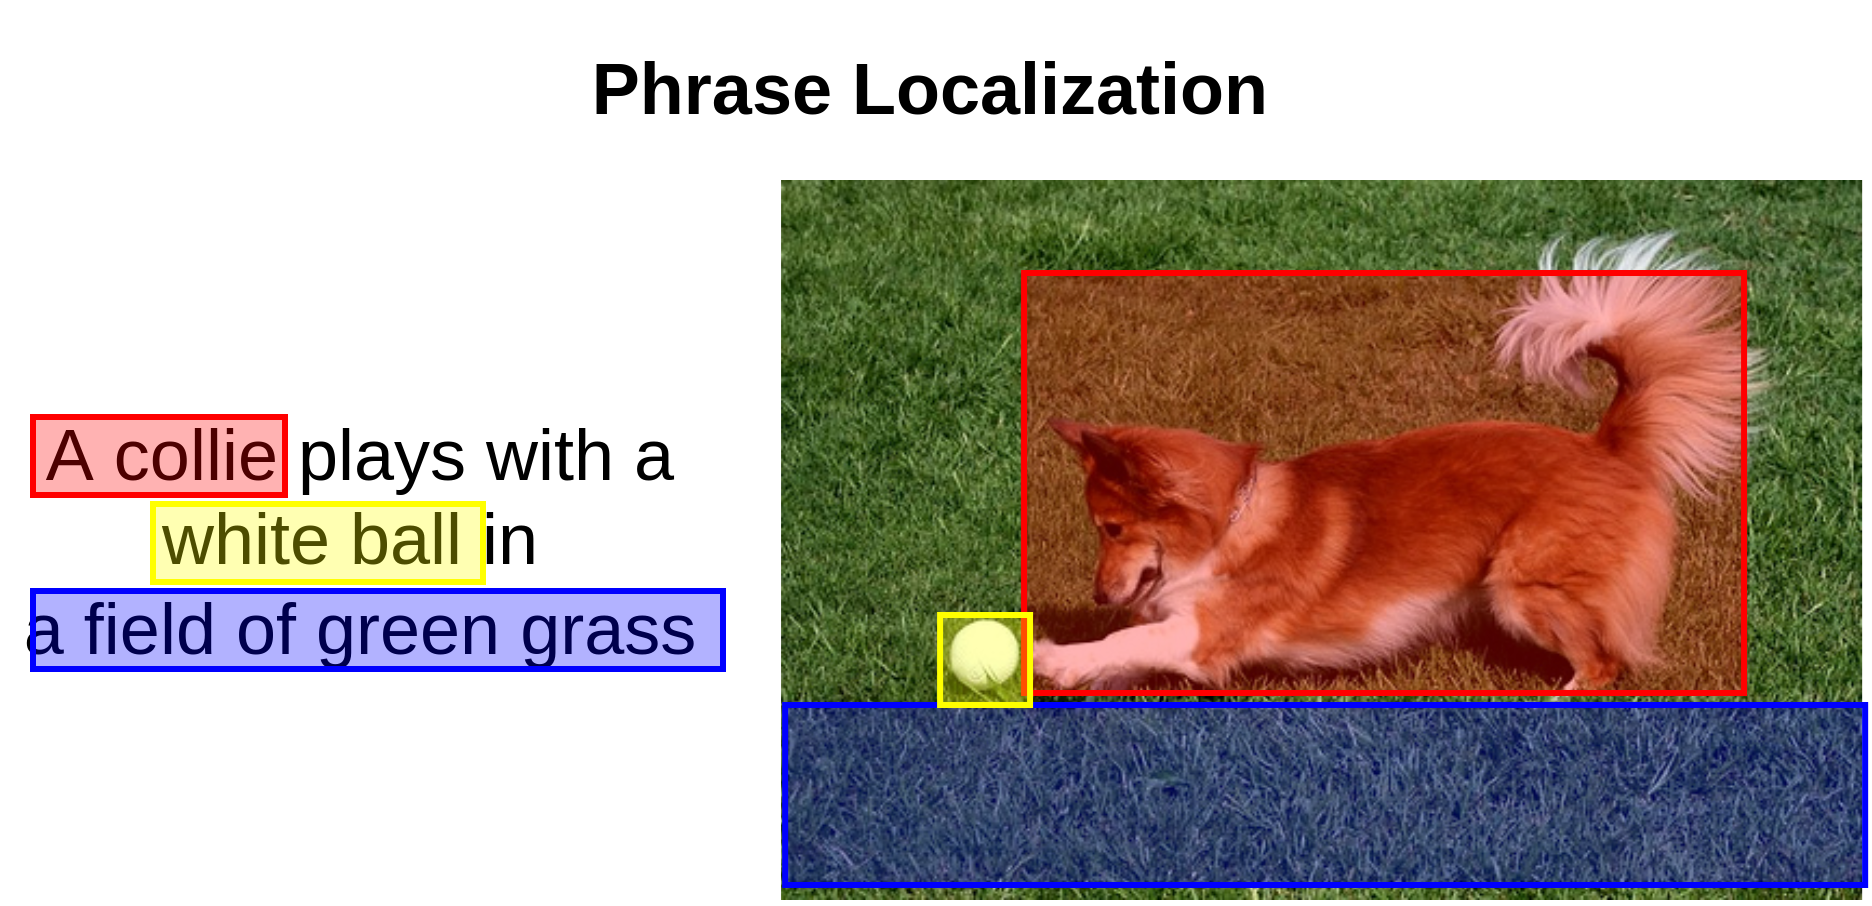
\includegraphics[width=7cm]{images/dog-playing-with-ball.png}

  \vspace{0.5cm}

  \begin{alertblock}{Def. (Phrase Grounding)}
    Attività di localizzazione del contenuto di un immagine referenziato da una
    frase.
  \end{alertblock}
\end{frame}

\section{Motivazione}

\begin{frame}{Motivazione e sfide}
  \begin{columns}
    \column{0.50\linewidth}
      \begin{itemize}
        \item Tassello fondamentale per diversi task in computer vision
        come 
        \begin{itemize} 
          \item \alert{visual question answering}, 
          \item \alert{image retrieval}, e 
          \item \alert{robotic navigation}
        \end{itemize}
      \end{itemize}
    \column{0.50\linewidth}
      \begin{itemize}
        \item Necessarie \alert{moltissime annotazioni}
        \item Utilizziamo la \alert{supervisione debole} (weak)
      \end{itemize}
      \vspace{0.5cm}
      \centering
      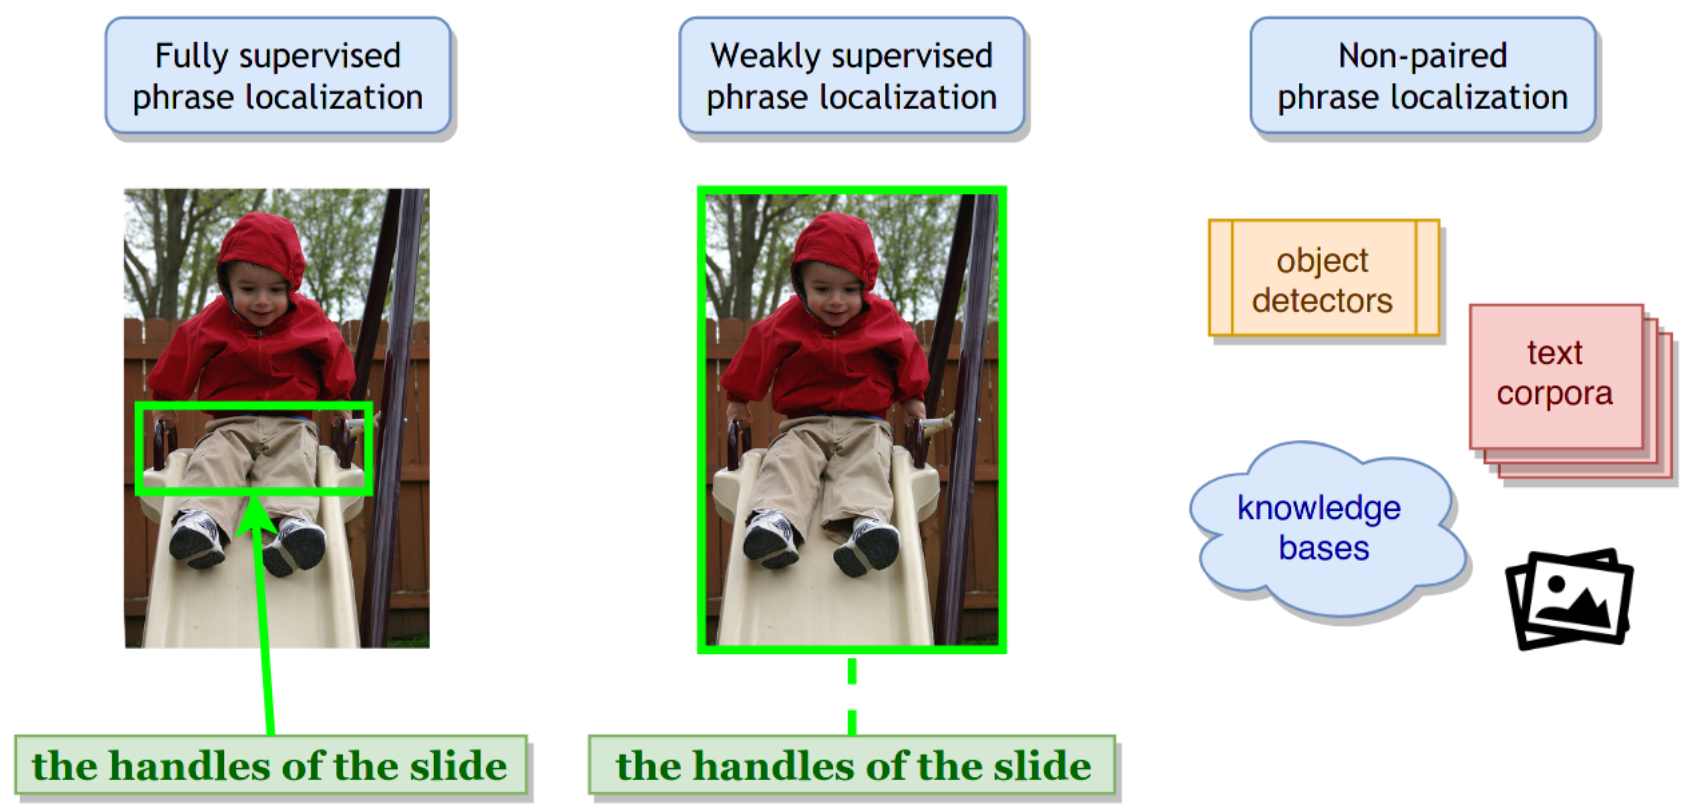
\includegraphics[width=5cm]{images/full-weak-no-supervision.png}
  \end{columns}
\end{frame}

\section{Stato dell'arte}

\begin{frame}{Approcci weakly supervised}
  \begin{itemize}
    \item Sfruttare l'informazione contenuta nella \alert{struttura
    della frase}
    \item Riformulare il problema del phrase grounding sotto forma del
    task \alert{image retrieval}
    \item \alert{Ricostruire} le features originali partendo da un
    codice (encoder-decoder)
    \item Apprendere una rappresentazione tramite
    \alert{attrazione e repulsione} delle features
  \end{itemize}
\end{frame}

\section{La nostra soluzione}

\begin{frame}{La nostra soluzione}
  \begin{itemize}
    \item Sfruttare informazione aggiuntiva dell'object detector (per
    ogni proposal restituisce una \alert{distribuzione di probabilità}
    su un set di classi)
    \item Le classi esprimono il \alert{contenuto semantico} delle
    proposal
    \vspace{0.5cm}
    \begin{alertblock}{Assunzione}
      Data una frase e una proposal, è più probabile che vi sia
      grounding tra le due se la \alert{similarità} tra la frase e la
      classe della proposal è alta
    \end{alertblock}
    \vspace{0.5cm}
    \item Il modello utilizza \alert{tre input}: modalità visuale,
    modalità testuale e similarità di concetto 
  \end{itemize}
\end{frame}

\begin{frame}{Visual Branch}
  \begin{columns}
    \column{0.50\linewidth}
      \begin{itemize}
        \item Object detector estrae dall'immagine $k$ proposal e per
        ognuna un vettore di \alert{features visuali}
        \item Aggiungiamo cinque \alert{features spaziali} (coordinate e
        area della proposal)
        \item \alert{Proiezione} delle features ne riduce la dimensionalità
      \end{itemize}
    \column{0.50\linewidth}
      \centering
      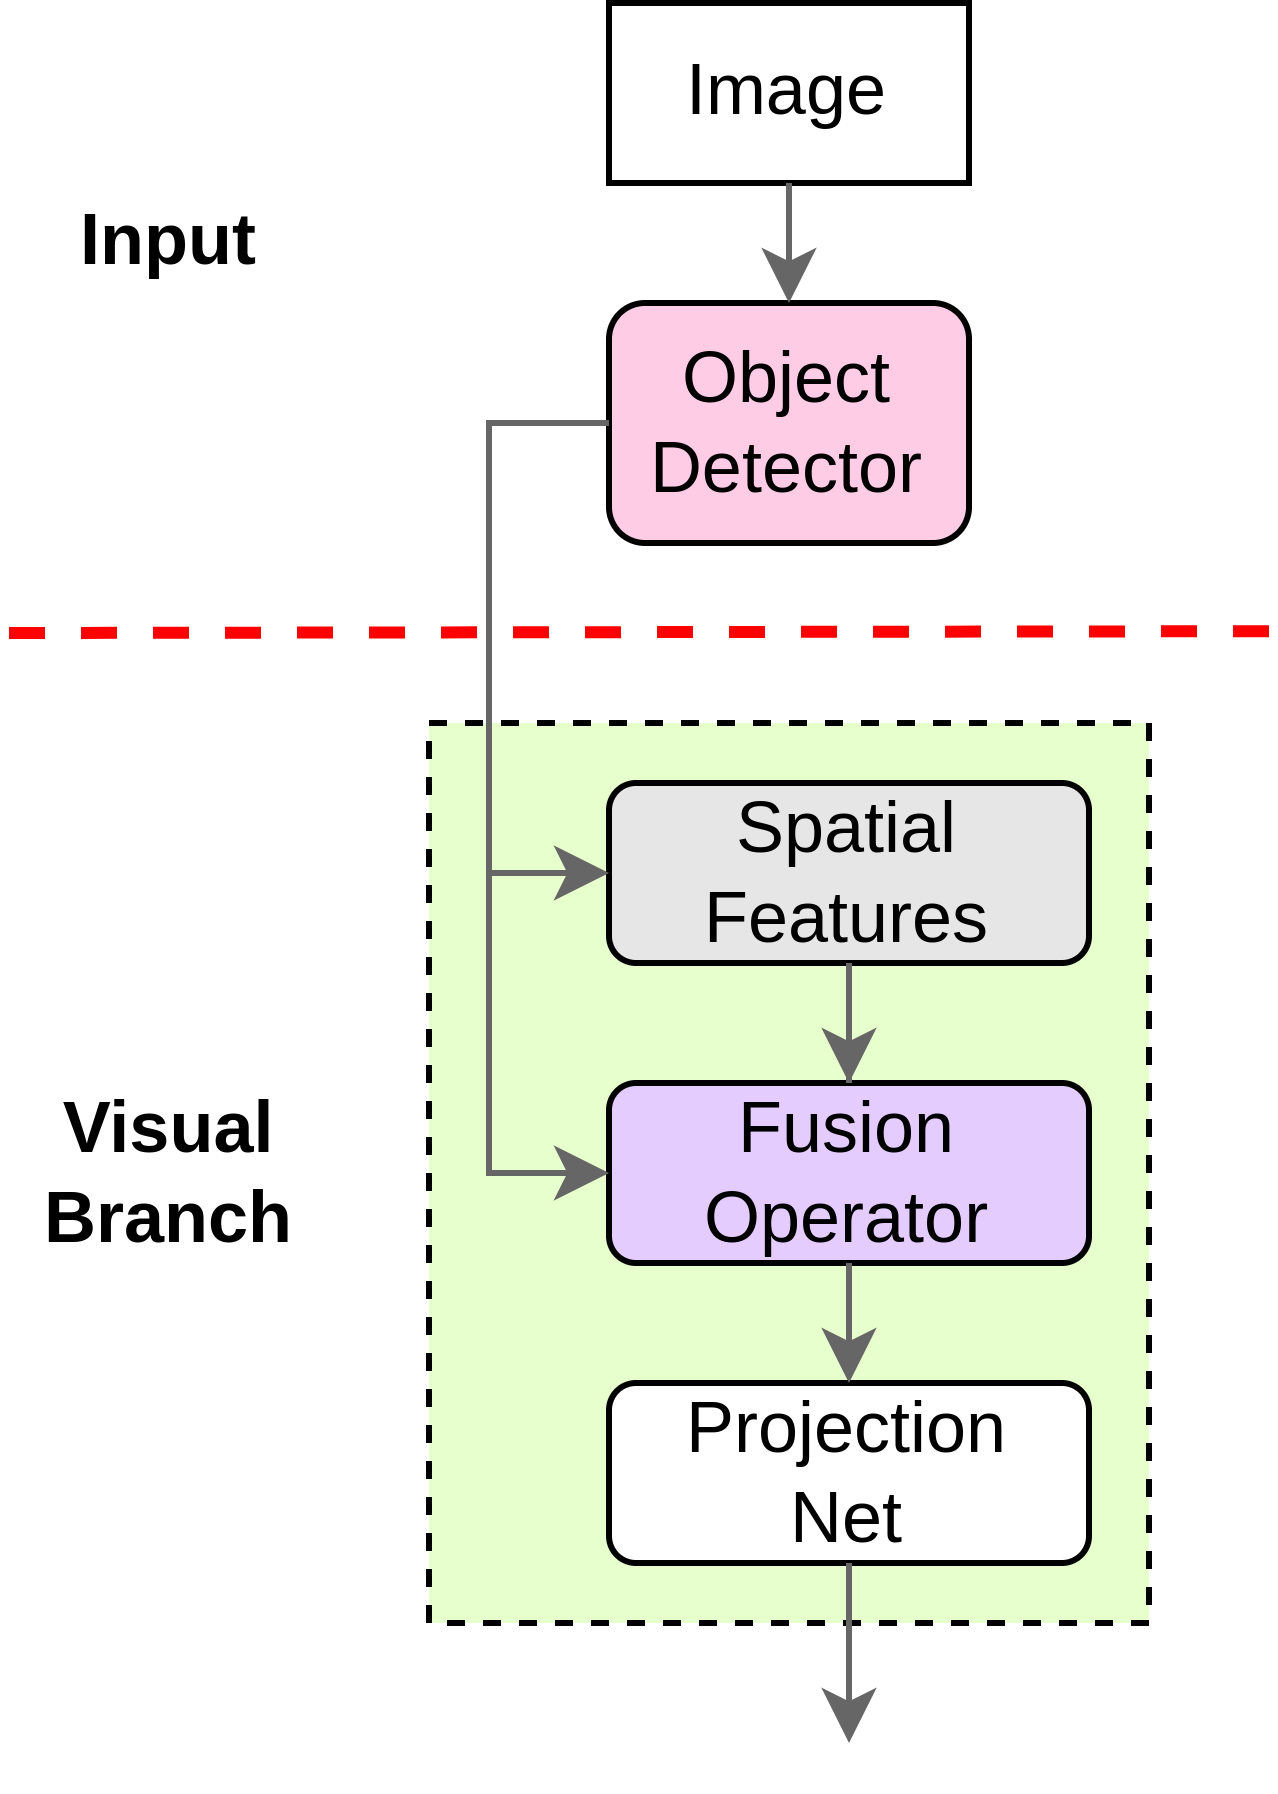
\includegraphics[width=3.5cm]{images/visual-branch.png}
  \end{columns}
\end{frame}

\begin{frame}{Textual Branch}
  \begin{columns}
    \column{0.50\linewidth}
      \begin{itemize}
        \item Calcoliamo il \alert{word embedding} di ogni parola nella query
        \item Codifichiamo la \alert{sequenza} di parole tramite una LSTM
        \item Utiliziamo l'output ottenuto per \alert{l'ultima} parola
      \end{itemize}
    \column{0.50\linewidth}
      \centering
      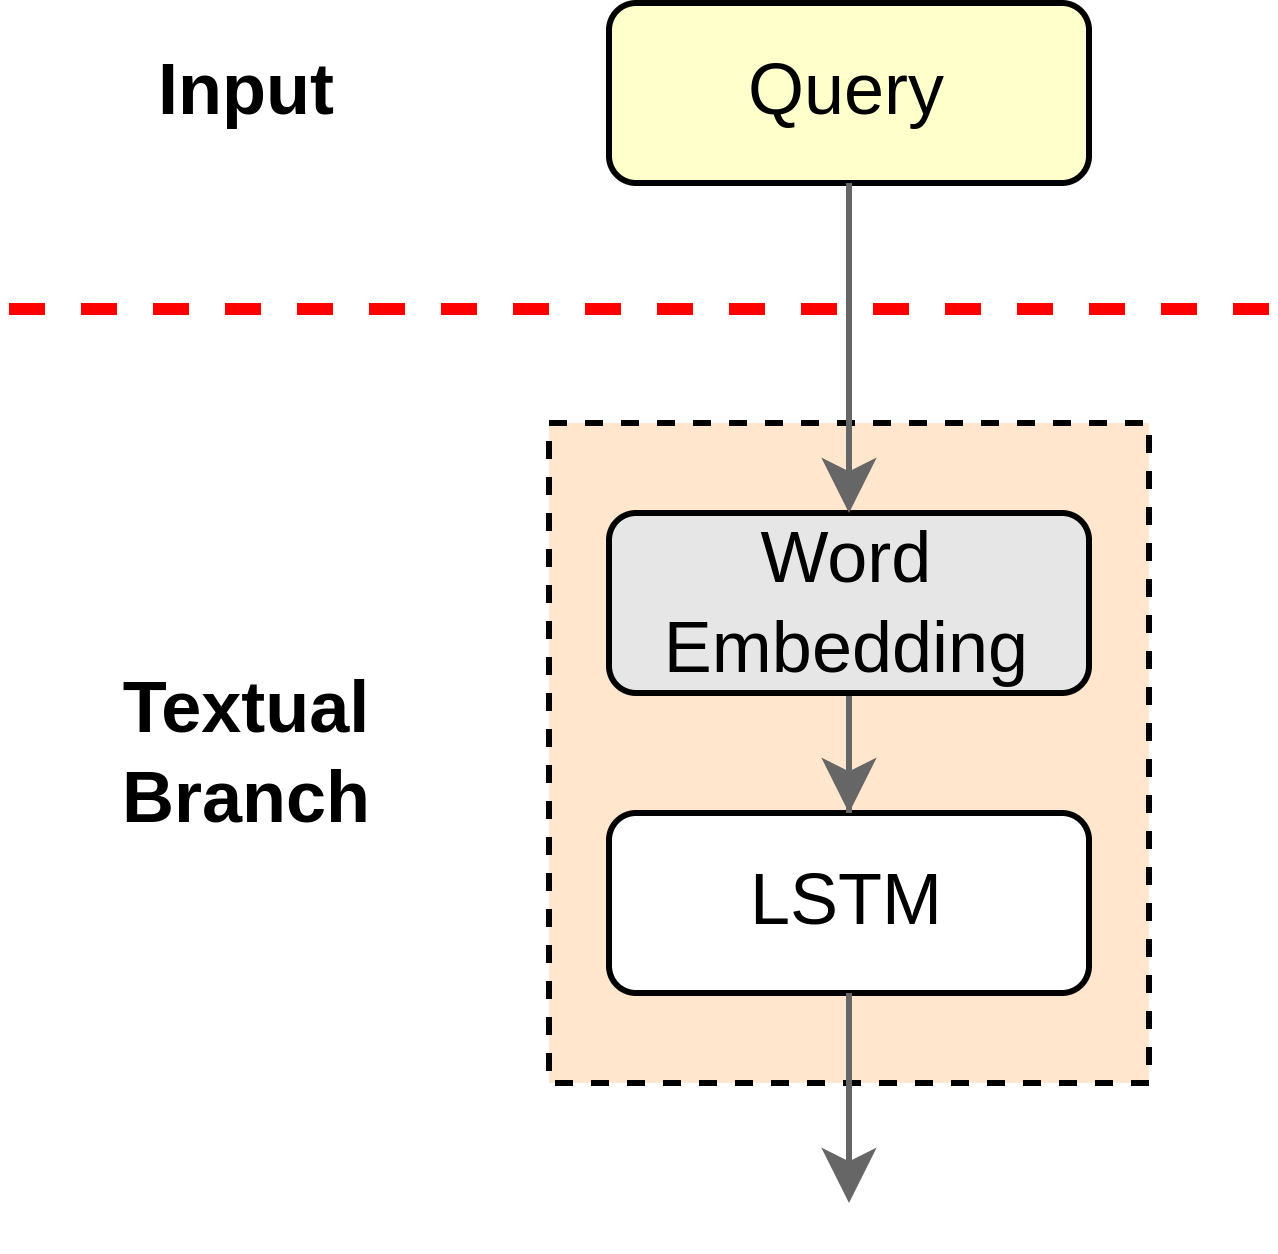
\includegraphics[width=3.5cm]{images/textual-branch.png}
  \end{columns}
\end{frame}

\begin{frame}{Concept Branch}
  \begin{columns}
    \column{0.50\linewidth}
      \begin{itemize}
        \item Selezioniamo il \alert{concetto} della frase come la
        \alert{parola} con similarità più alta rispetto alle classi
        delle proposal
        \item Concept Similarity = similarità tra \alert{l'embedding del
        concetto} della frase e \alert{l'embedding della classe} di ogni
        proposal
      \end{itemize}
    \column{0.50\linewidth}
      \centering
      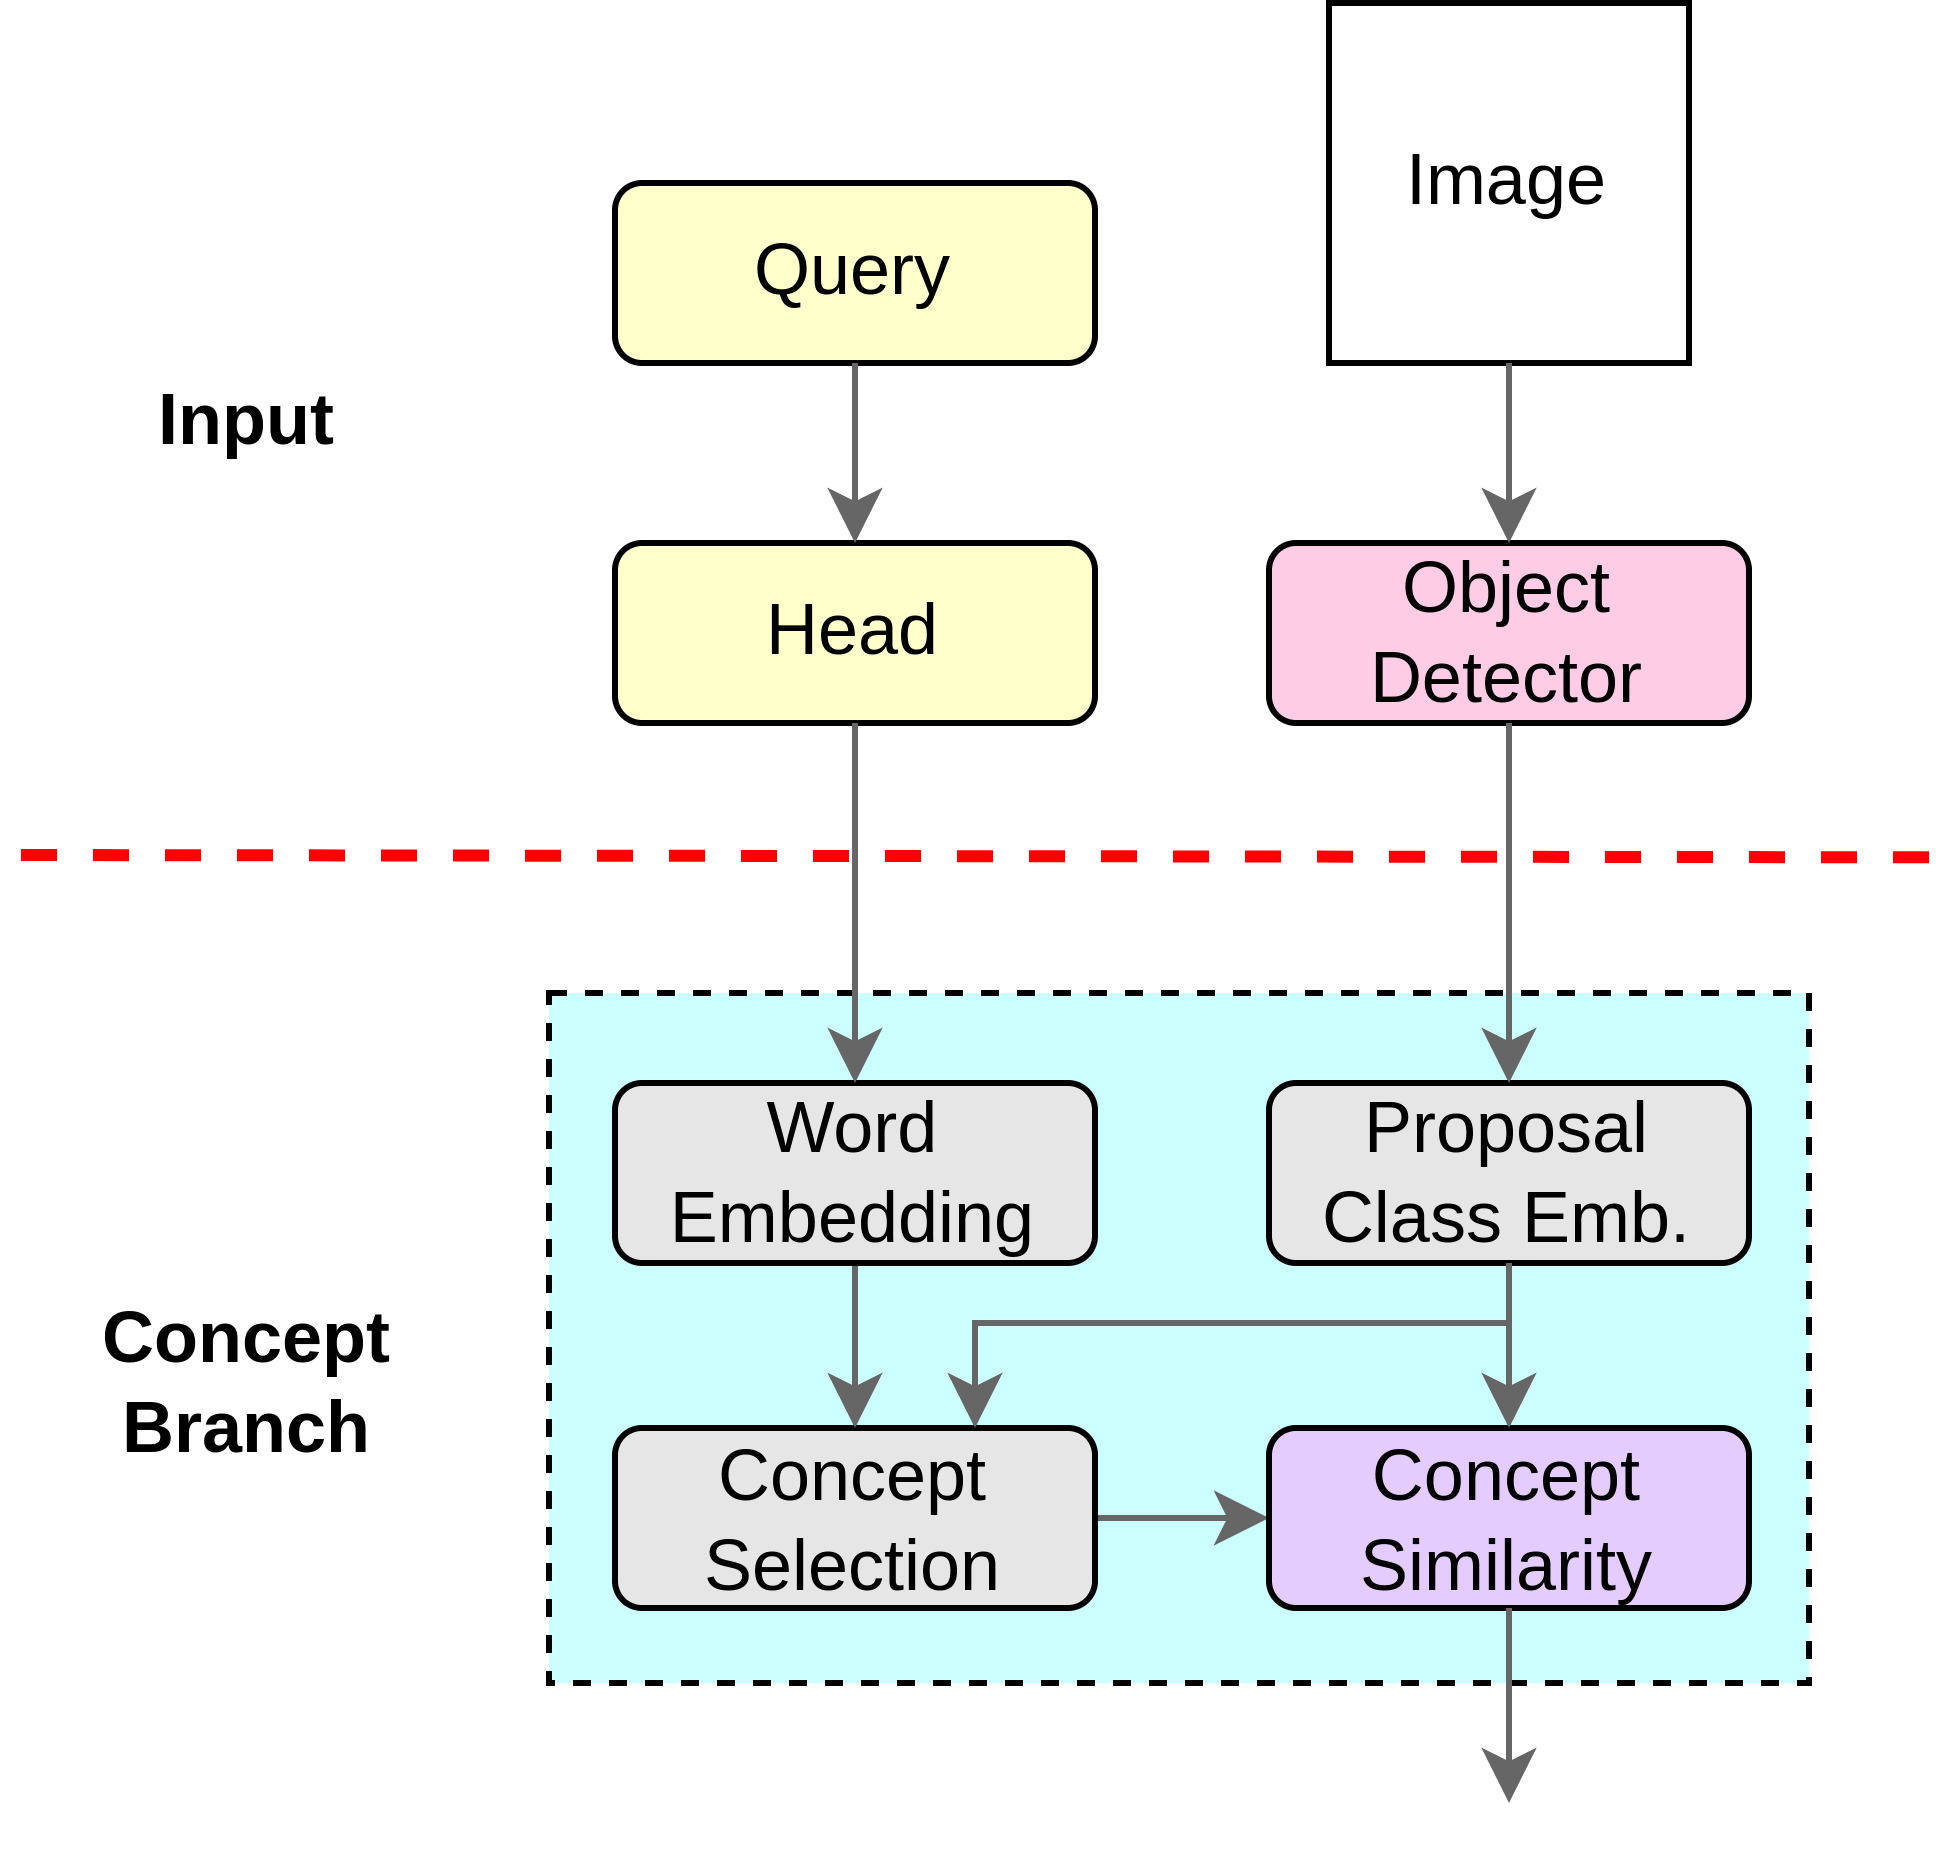
\includegraphics[width=4.5cm]{images/concept-branch.png}
  \end{columns}
\end{frame}

\begin{frame}{Concept Selection}
  \centering
  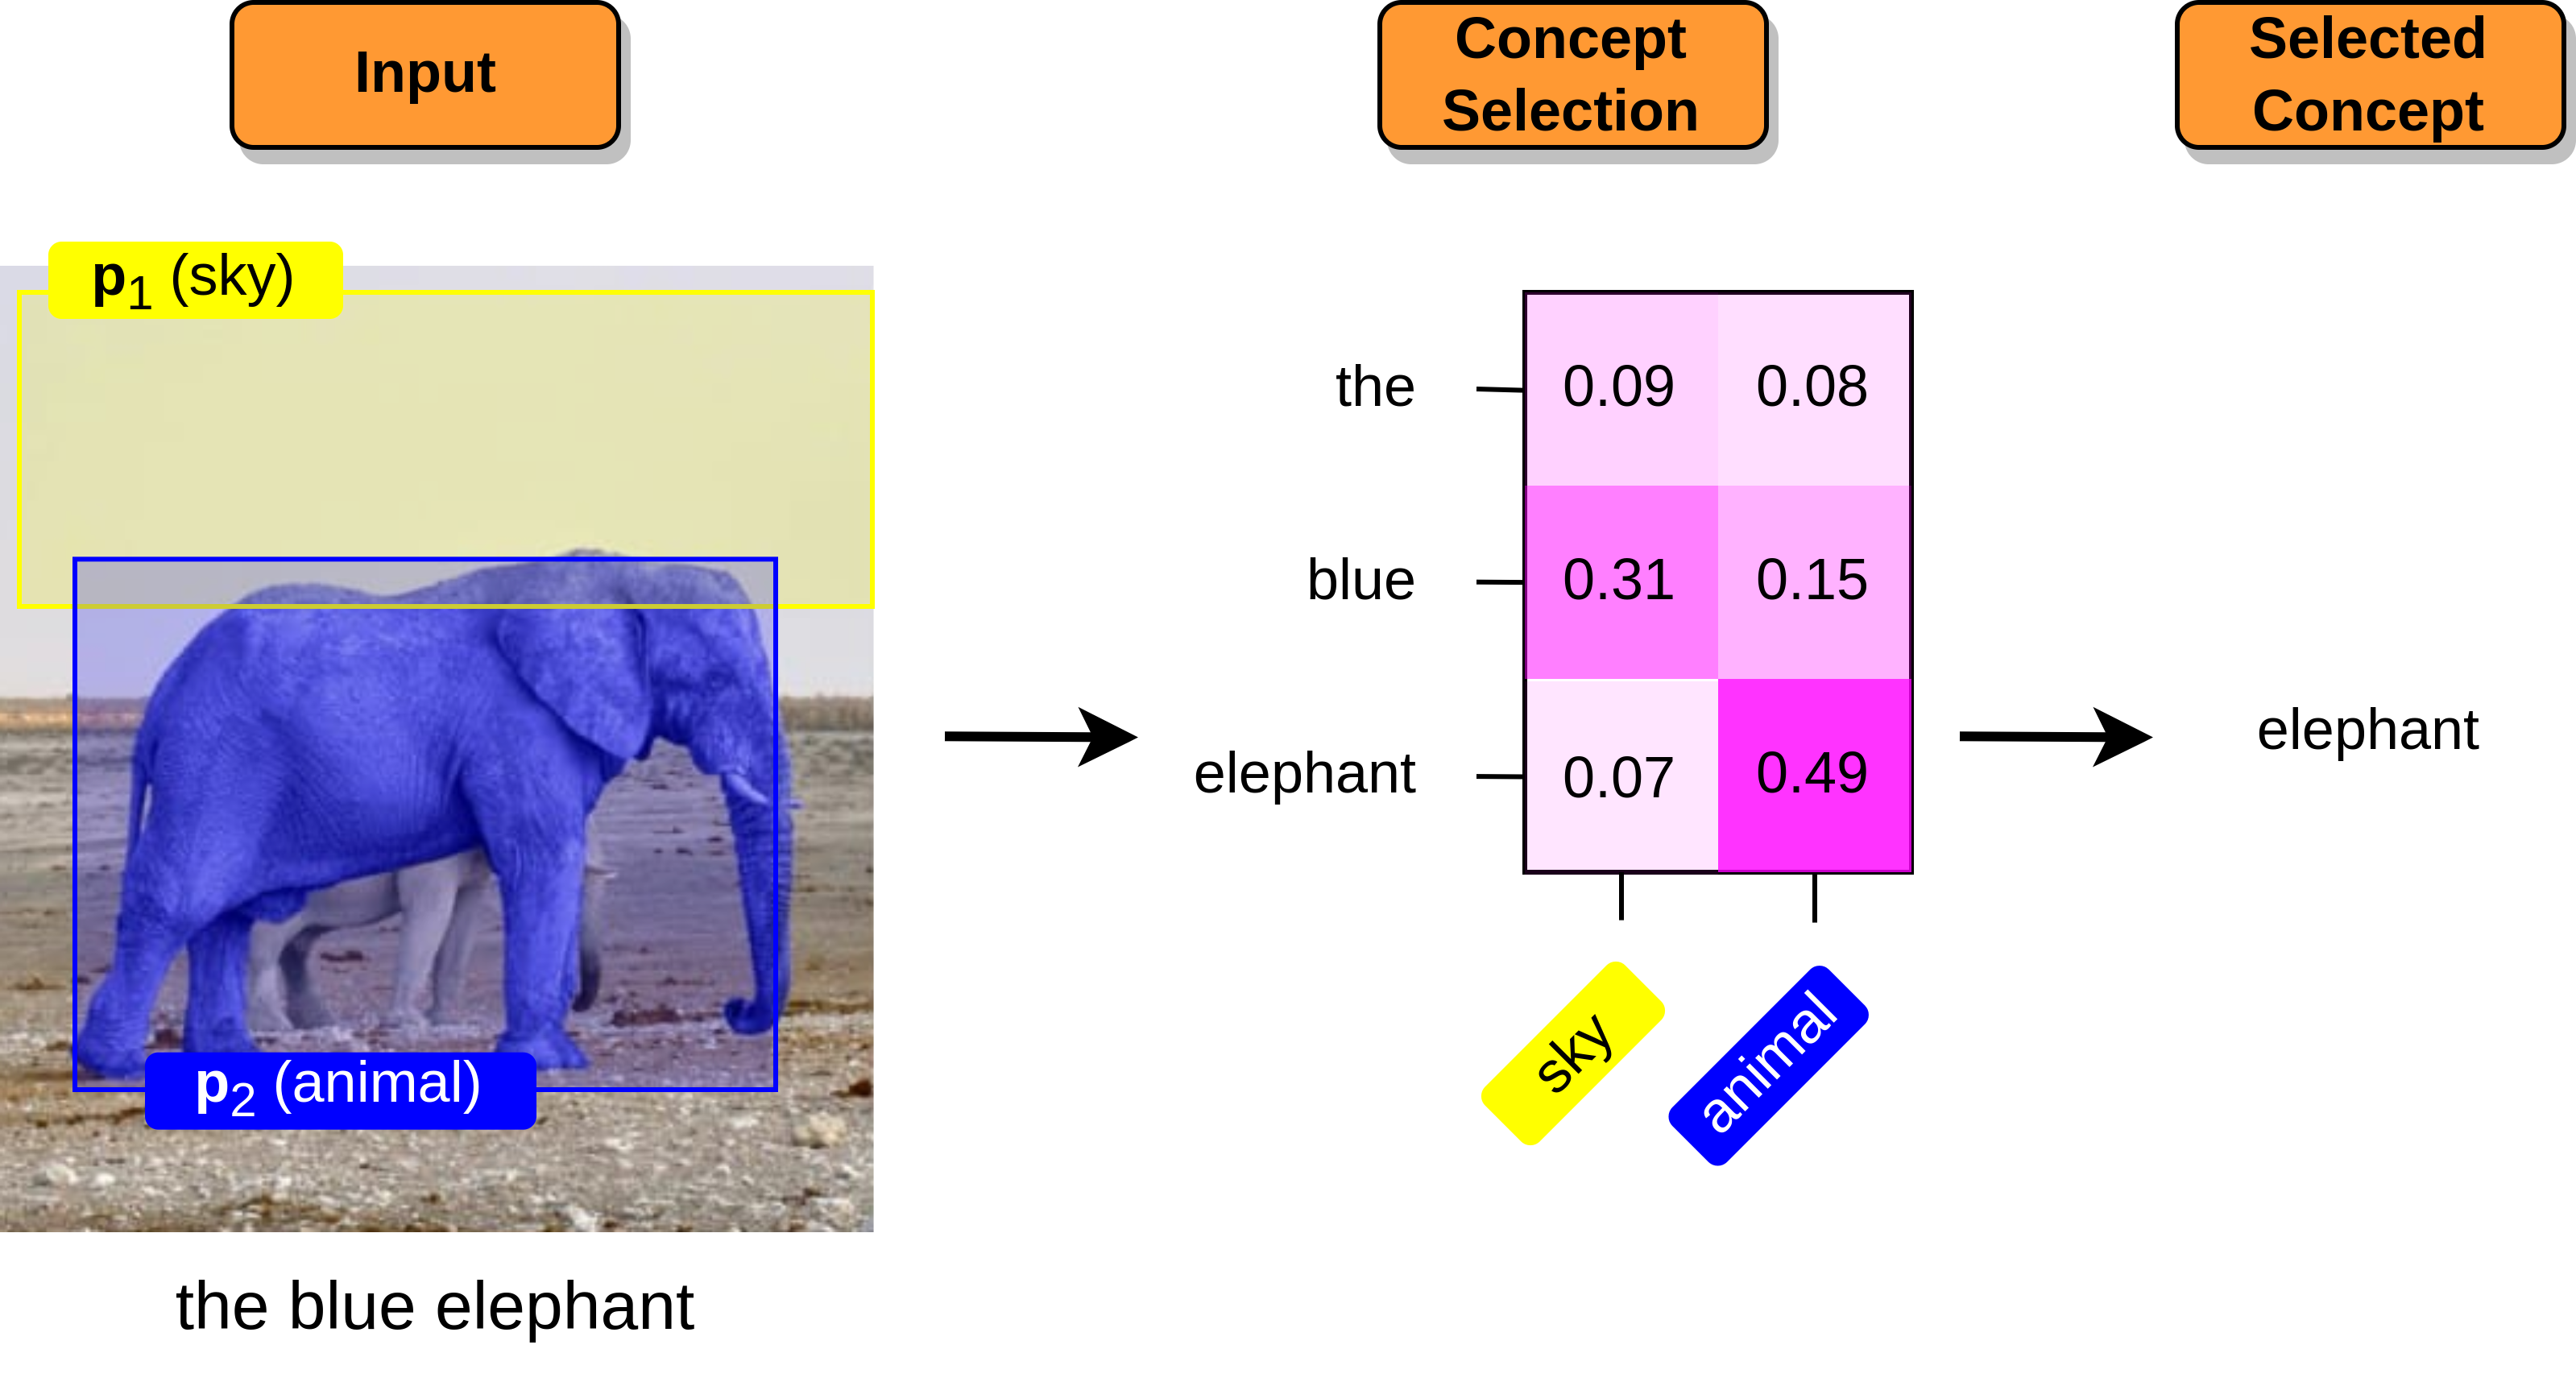
\includegraphics[width=9cm]{images/concept-selection-example.png}
\end{frame}

\begin{frame}{Predizioni}
  \begin{itemize}
    \item Predizioni calcolate come uno \alert{score di similarità}
    tra la modalità visiva e quella testuale
    \item Alle predizioni viene applicata la concept similarity come
    \alert{Media pesata} tra i due score di similarità
    \item In fase di inferenza, per ogni frase nominale il modello
    restituisce la \alert{proposal con score massimo}
  \end{itemize}

  \vspace{0.5cm}

  \centering
  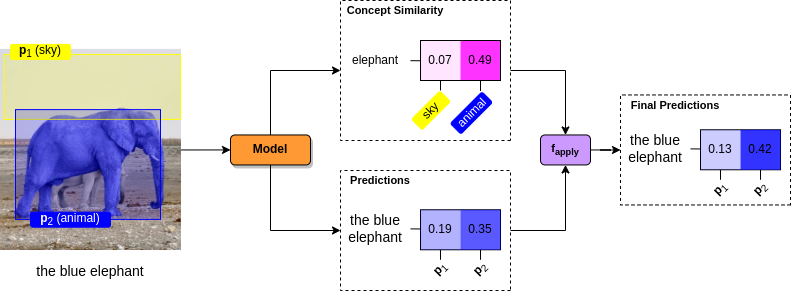
\includegraphics[width=9cm]{images/predictions.png}
\end{frame}

\begin{frame}{Architettura}
  \centering
  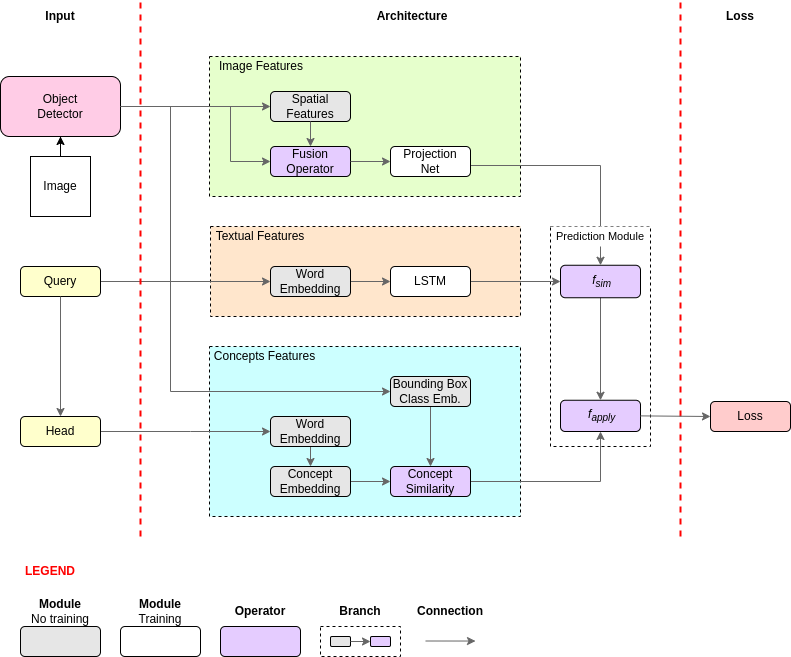
\includegraphics[width=9cm]{images/model-architecture.png}
\end{frame}

\begin{frame}{Similarità Multimodale}
  La similarità multimodale rappresenta la \alert{similarità aggregata
  tra immagine e frase}, condizionata dalle frasi nominali (noun
  phrases) \vspace{1cm}

  \centering
  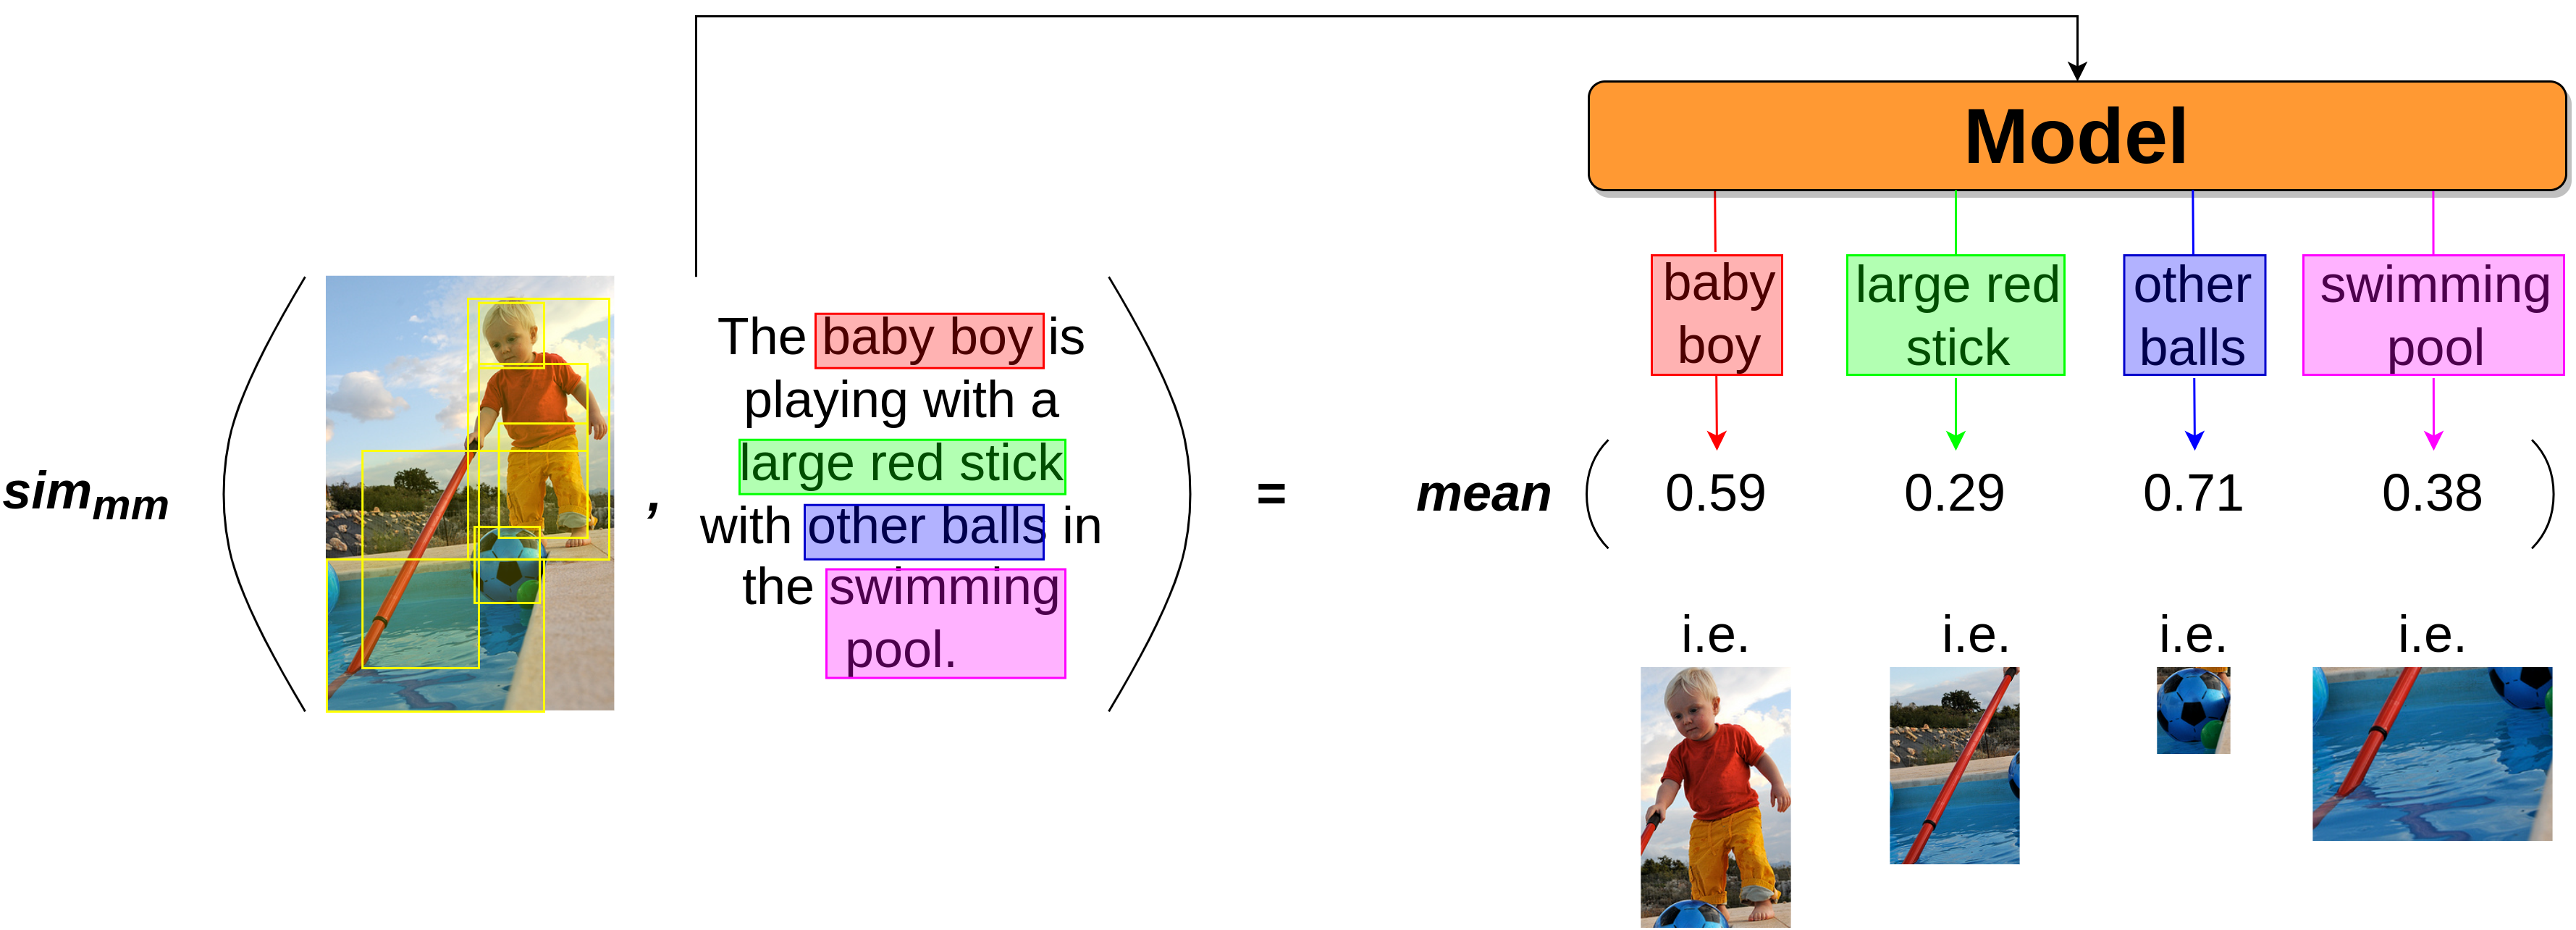
\includegraphics[width=9cm]{images/sim-mm.png}
\end{frame}

\begin{frame}{Loss}
  Fissata un'immagine $\bm{I}$, due frasi $\text{S}$ e $\text{S}'$
  dove $\text{S}$ descrive $\bm{I}$ mentre $\text{S}'$ \textbf{non}
  descrive $\bm{I}$:
  \begin{itemize}
    \item \alert{Massimizziamo} la similarità multimodale tra $\bm{I}$
    e $\text{S}$
    \item \alert{Minimizziamo} la similarità multimodale tra $\bm{I}$
    e $\text{S}'$
  \end{itemize}
  
  \vspace{0.5cm}

  \centering
  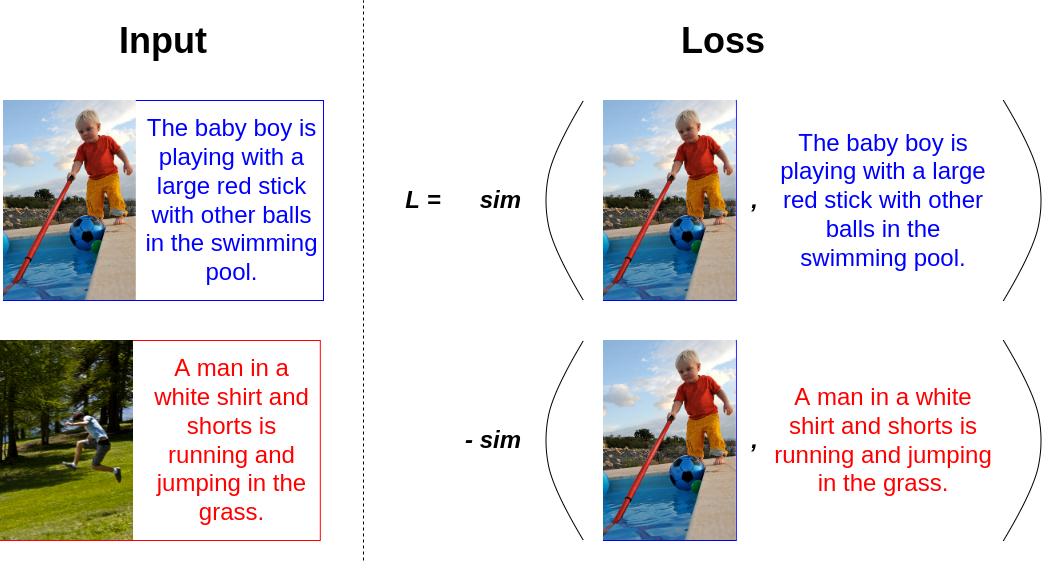
\includegraphics[width=7cm]{images/loss.png}
\end{frame}

\section{Risultati}

\begin{frame}{Risultati Quantitativi (Flickr30k Entities)}
  \centering
  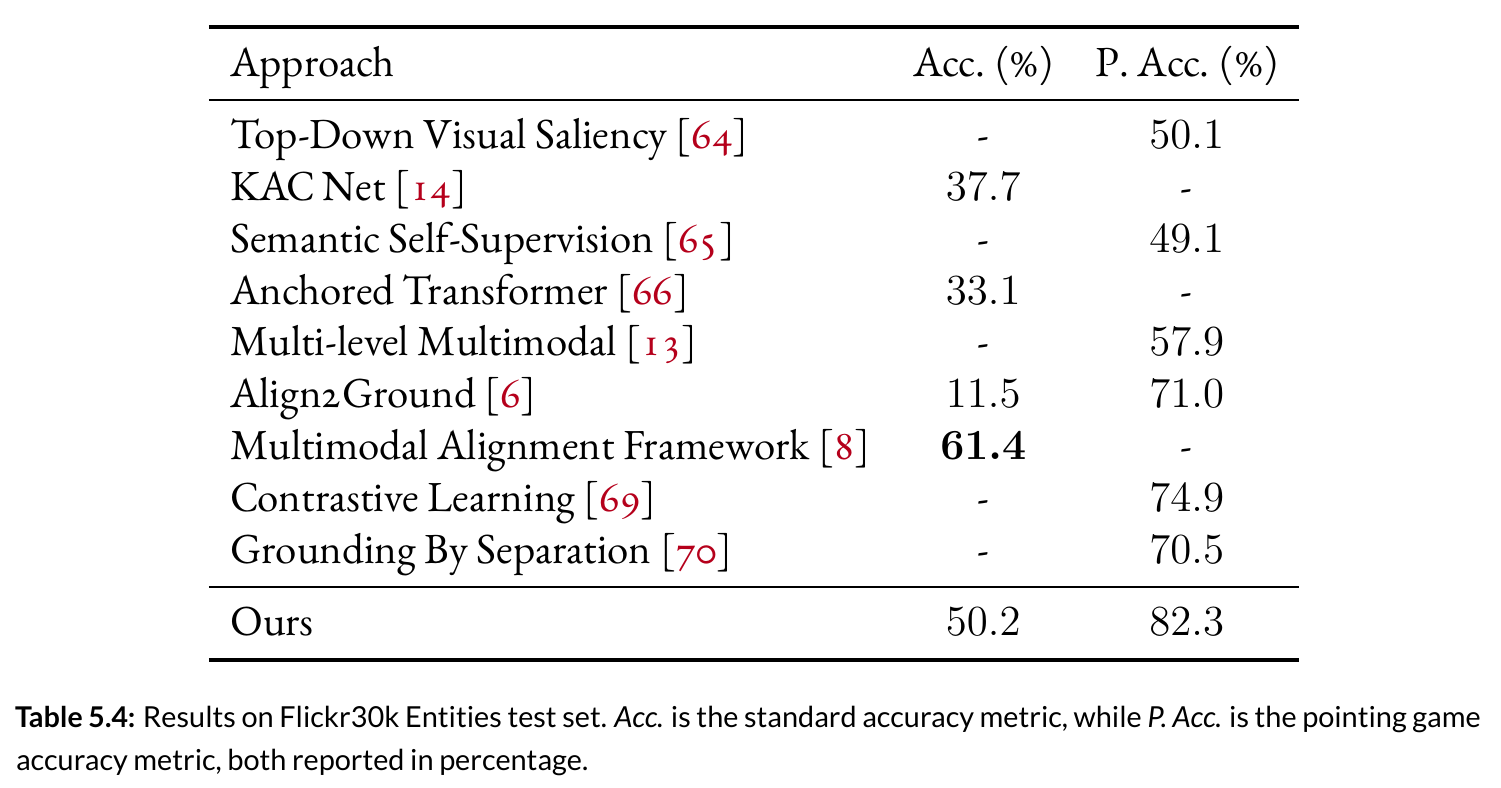
\includegraphics[width=9cm]{images/flickr30k-results.png}
\end{frame}

\begin{frame}{Risultati Quantitativi (ReferIt)}
  \centering
  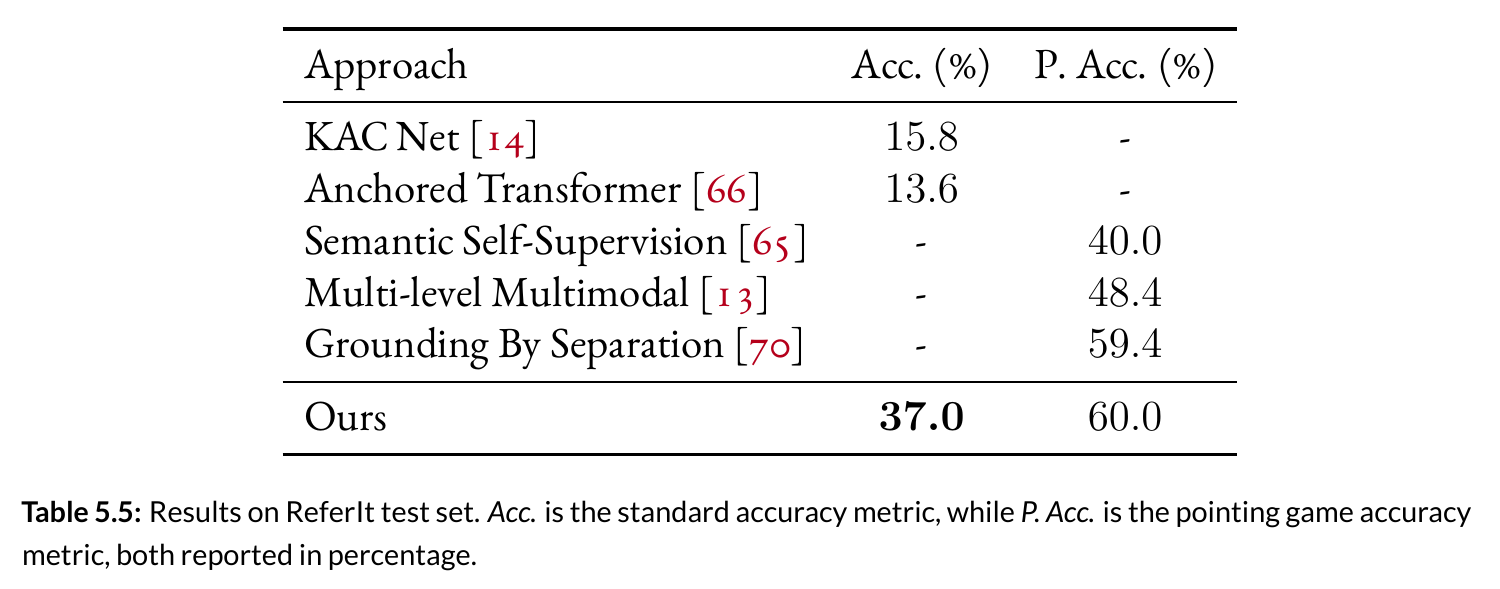
\includegraphics[width=9cm]{images/referit-results.png}
\end{frame}

\begin{frame}{Risultati Qualitativi}
  \centering
  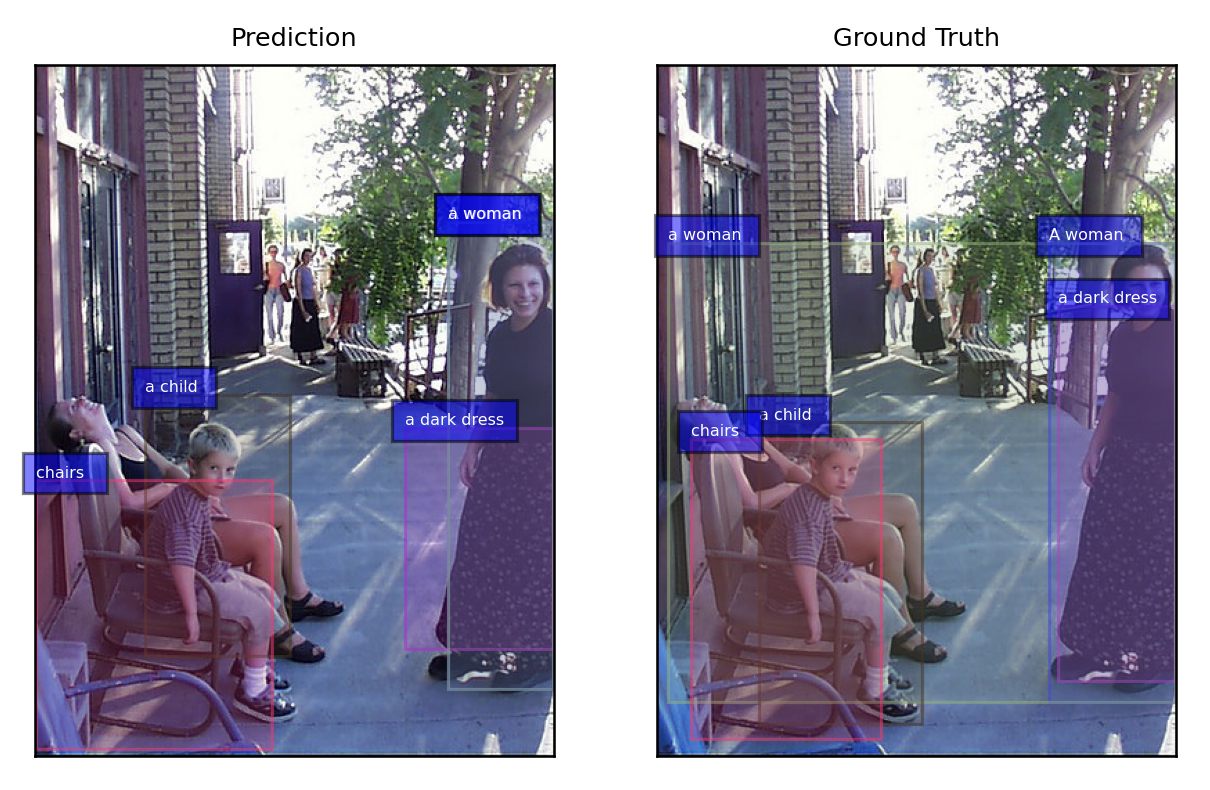
\includegraphics[width=9cm]{images/similing-woman.png}
  
  ``\underline{A woman} in \underline{a dark dress} smiles while
  \underline{a woman} across from her and \underline{a child} sit in
  \underline{chairs}''
\end{frame}

\section{Conclusioni}

\begin{frame}{Conclusioni e lavori futuri}
  \begin{columns}
    \column{0.50\linewidth}
      \textbf{Conclusioni}
      \begin{itemize}
        \item Anche con un \alert{modello semplice}, la concept
        similarity ci ha permesso di raggiungere \alert{risultati
        comparabili} allo stato dell'arte
      \end{itemize}
    \column{0.50\linewidth}
      \textbf{Lavori Futuri}
      \begin{itemize}
        \item \alert{Evitare} di apprendere \alert{rappresentazioni
        visive che mimano quelle testuali} (e vice-versa), forzate
        dalla misura di similarità
        \item Considerare gli \alert{attributi} delle proposal per
        \alert{disambiguare le predizioni} relative a frasi simili
        (stesso concetto)
      \end{itemize}
  \end{columns}
\end{frame}

\begin{frame}
  \centering
  \huge
  Grazie per l'attenzione!
\end{frame}

\end{document}
